%==============================================================================
%  Standalone PREVIEW v2 of the "DataSAIL baseline" poster block — improved
%  3-step workflow diagram (glyphs + red-coded failure steps + scaling wall).
%  Does NOT touch lowrank_poster.tex. Compile: pdflatex datasail_block_preview_v2.tex
%==============================================================================
\documentclass{article}
\usepackage[paperwidth=35cm, paperheight=20cm, margin=1cm]{geometry}
\usepackage[T1]{fontenc}
\usepackage[utf8]{inputenc}
\usepackage{helvet}
\renewcommand{\familydefault}{\sfdefault}
\usepackage{amsmath, amssymb}
\usepackage{tikz}
\usepackage{pifont}
\usepackage{xcolor}
\usetikzlibrary{arrows.meta, positioning, calc}
\pagestyle{empty}

%---- palette (copied from lowrank_poster.tex) ------------------------------
\definecolor{maroon}{HTML}{7A0C00}
\definecolor{ink}{HTML}{14243B}
\definecolor{blue}{HTML}{2563EB}
\definecolor{green}{HTML}{1B7A3D}
\definecolor{soft}{HTML}{F3F0EC}
\definecolor{softblue}{HTML}{EAF1FE}
\definecolor{rulec}{HTML}{D9C7C2}
\color{ink}

%---- macros (copied from lowrank_poster.tex) -------------------------------
\newcommand{\pblock}[1]{%
  \par\vspace{1.6ex}%
  \begin{center}{\color{maroon}\bfseries\Large #1}\end{center}%
  \vspace{-1.0ex}{\color{rulec}\rule{\linewidth}{1.3pt}}\par\vspace{0.6ex}}
\newcommand{\callout}[2]{%
  \begin{center}\colorbox{#1}{\begin{minipage}{0.93\linewidth}\vspace{0.5ex}
  #2\vspace{0.5ex}\end{minipage}}\end{center}}

\begin{document}
\noindent\begin{minipage}{33cm}

\pblock{The baseline: DataSAIL}
{\large \textbf{DataSAIL}\ {\footnotesize(\emph{Data Splitting Against
Information Leakage})}\ is the standard leakage-aware splitter and our closest
baseline. It targets the \emph{same} cross-split similarity — but solves it
\textbf{exactly}, and every step is $O(n^2)$ or worse:}
\vspace{1.2ex}
\begin{center}
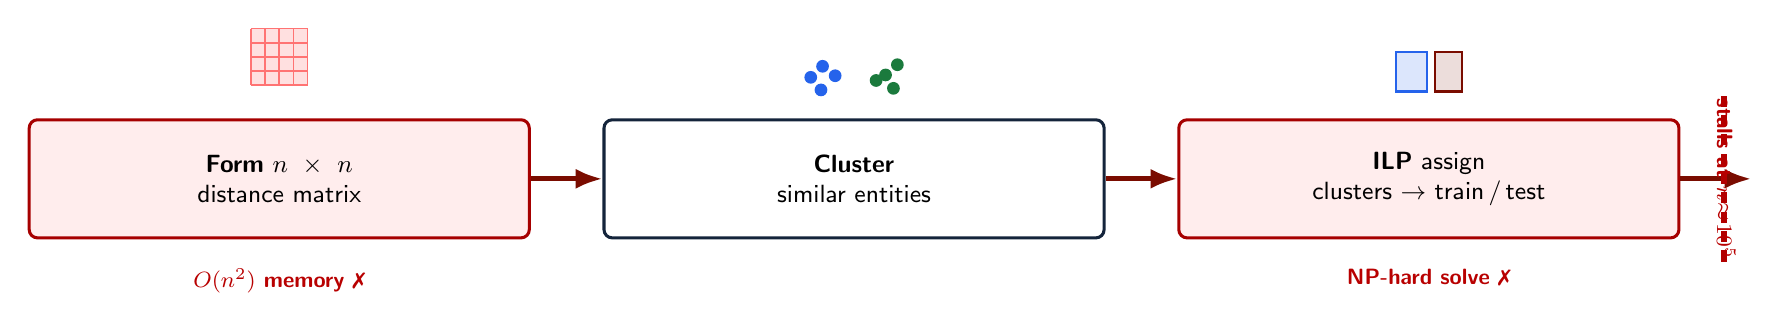
\begin{tikzpicture}[font=\small,
   b/.style   ={rectangle, rounded corners=3pt, line width=1.1pt, align=center,
                inner sep=5pt, minimum height=15mm, text width=6.0cm},
   bad/.style ={b, draw=red!65!black, fill=red!7},
   ok/.style  ={b, draw=ink, fill=white},
   ar/.style  ={-{Latex[length=3.4mm]}, line width=1.7pt, draw=maroon},
   cost/.style={red!72!black, font=\footnotesize\bfseries}]

 % ---- step boxes -----------------------------------------------------------
 \node[bad] (d) at (0,0)    {\textbf{Form} $n\times n$\\ distance matrix};
 \node[ok]  (c) at (7.3,0)  {\textbf{Cluster}\\ similar entities};
 \node[bad] (i) at (14.6,0) {\textbf{ILP} assign\\ clusters $\to$ train\,/\,test};
 \draw[ar] (d)--(c);  \draw[ar] (c)--(i);

 % ---- glyphs above each step ----------------------------------------------
 % n x n grid (dense distance matrix)
 \begin{scope}[shift={($(d.north)+(-0.36,0.42)$)}]
   \fill[red!12] (0,0) rectangle (0.72,0.72);
   \foreach \k in {0,...,4}{\draw[red!55, line width=0.6pt] (\k*0.18,0)--(\k*0.18,0.72);
                            \draw[red!55, line width=0.6pt] (0,\k*0.18)--(0.72,\k*0.18);}
 \end{scope}
 % two clusters of dots
 \begin{scope}[shift={($(c.north)+(0,0.5)$)}]
   \foreach \p in {(-0.55,0.02),(-0.4,0.16),(-0.42,-0.14),(-0.24,0.04)}{\fill[blue]\p circle(2.3pt);}
   \foreach \p in {(0.4,0.05),(0.55,0.18),(0.5,-0.12),(0.28,-0.02)}{\fill[green]\p circle(2.3pt);}
 \end{scope}
 % two split bins
 \begin{scope}[shift={($(i.north)+(-0.42,0.34)$)}]
   \fill[blue!16]  (0,0) rectangle (0.4,0.5); \draw[blue,line width=0.8pt] (0,0) rectangle (0.4,0.5);
   \fill[maroon!14](0.5,0) rectangle (0.84,0.5); \draw[maroon,line width=0.8pt] (0.5,0) rectangle (0.84,0.5);
 \end{scope}

 % ---- cost tags under the failing steps -----------------------------------
 \node[cost, below=2.5mm of d] {$O(n^2)$ memory \ding{55}};
 \node[cost, below=2.5mm of i] {NP-hard solve \ding{55}};

 % ---- scaling wall ---------------------------------------------------------
 \draw[ar] (i.east) -- ++(0.9,0);
 \draw[red!70!black, line width=2.4pt, dash pattern=on 4pt off 3pt]
       (18.35,-1.05) -- (18.35,1.05);
 \node[red!72!black, font=\footnotesize\bfseries, rotate=-90, anchor=north]
       at (18.62,0) {stalls at $n\!\approx\!10^{5}$};
\end{tikzpicture}
\end{center}
\vspace{1.0ex}
\callout{softblue}{\centering\large Faithful but \textbf{unscalable}: it must
\emph{materialize} the whole $n\times n$ similarity and solve a combinatorial
program — \textbf{90\,min} at 100k, \textbf{out-of-memory} by 300k.
\textbf{This is the gap we factorize away.}}

\end{minipage}
\end{document}
